\begin{table}[t]
\captionsetup[subfigure]{aboveskip=-2pt, belowskip=-1pt}
\center
\caption{Summary of notation}\label{table:symbols}
\small
    \begin{tabular}{| p{1.2cm} | p{10cm} |}
        \hline
        Symbol & Description \\
        \hline
        \hline
        $\V{v}{i}$ & set of $i$-hop neighbors of vertex $v$ ($\V{v}{0} = \{ v \}$)\\
        $\LV{v}{i}$ & set of vertices that are at most $i$ hops away from vertex $v$ (i.e., $\LV{v}{i} = \cup_{k = 0}^{i} \V{v}{k}) $\\
        $\E{v}{i}$ & set of edges connecting two vertices in $\V{v}{i}$ ($\E{v}{0}$=$\emptyset$)\\
        $\LE{v}{i}$ & set of edges connecting two vertices in $\LV{v}{i}$\\
        \hline
    \end{tabular}
\end{table}
In this section, we define new terms that represent {\it multi-order ego networks} and {\it multi-order
friendship networks}, and then present several properties of the multi-order friendship networks.
Our betweenness computation algorithm in Section~\ref{sec:betweenness} takes advantage of these properties.

\begin{figure}[t]
        \captionsetup[subfigure]{aboveskip=-2pt, belowskip=-1pt}
        \centering
        \begin{subfigure}[b]{0.65\textwidth}
                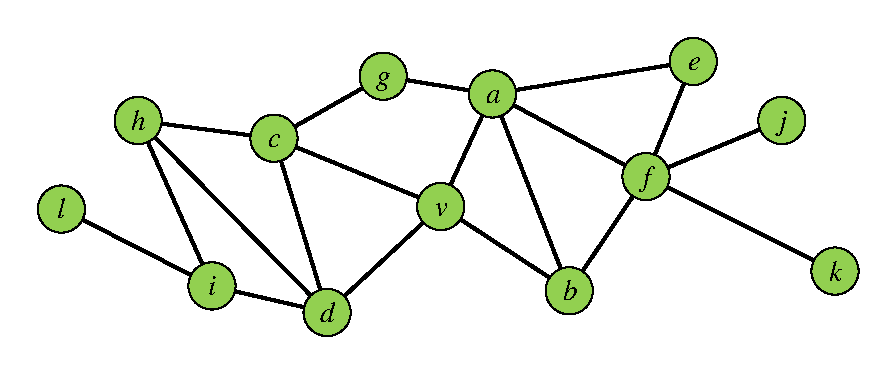
\includegraphics[width=\textwidth]{./images/figs-original.pdf}
                \caption{A given network}
                \label{fig:1-a}
        \end{subfigure}
        
        \begin{subfigure}[b]{0.3\textwidth}
                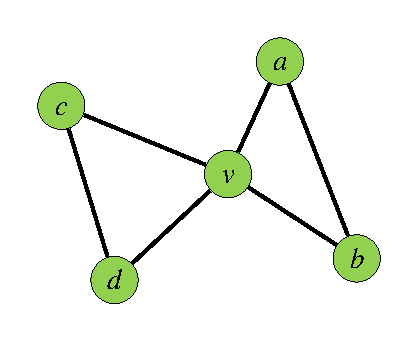
\includegraphics[width=\textwidth]{./images/ego2.pdf}
                \caption{Ego network}
                \label{fig:1-b}
        \end{subfigure}
        \begin{subfigure}[b]{0.5\textwidth}
                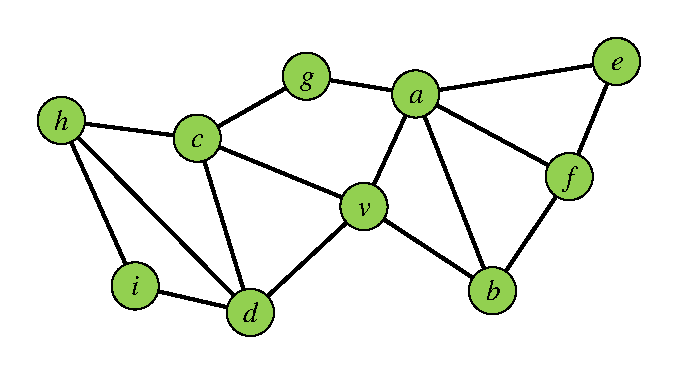
\includegraphics[width=\textwidth]{./images/second-order.pdf}
                \caption{Second-order ego network}
                \label{fig:1-c}
        \end{subfigure}
        \begin{subfigure}[b]{0.3\textwidth}
                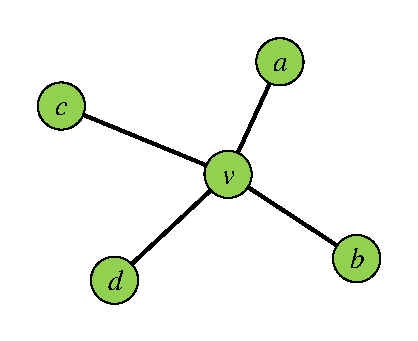
\includegraphics[width=\textwidth]{./images/friends.pdf}
                \caption{Friendship network}
                \label{fig:1-d}
        \end{subfigure}
        \begin{subfigure}[b]{0.5\textwidth}
                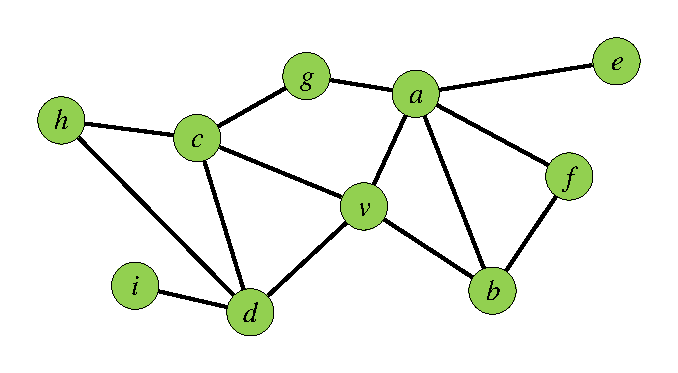
\includegraphics[width=\textwidth]{./images/multi-oder-friends.pdf}
                \caption{Second-order friendship network}
                \label{fig:1-e}
        \end{subfigure}
        \caption{The given network, and the $n$-order ego and friendship networks of vertex $v$}
        \label{fig:1}
\end{figure}

\subsection{Definitions}\label{subsec:x-egoDefinition}
In this paper, we consider a graph $G(V, E)$\footnote{We use the term {\em actors} and {\em social links} to refer to individuals, groups or organizations and their relationships in a social network. On the other hand, the graph representing a social network consists of {\em vertices} and {\em edges} representing actors and social links, respectively.} where $V$ is a set of vertices and $E$ is a set of undirected edges representing social links between vertices.
In the literature~\cite{egocentric, everett, ICCN:lbcdna, SIMBET}, given a graph $G(V, E)$ and a vertex $v \in V$, the {\em ego network} of $v$ is defined as the subgraph of $G$ consisting of $v$ and its 1-hop neighbors (i.e., vertices with an edge to $v$) as well as the edges between these vertices.
Using the notation summarized in Table~\ref{table:symbols}, this ego network can be formally extended to \emph{$n$-order ego network} as follows:

\begin{definition}\label{def:multi-order-ego-network}
Given a graph $G(V, E)$ and a vertex $v \in V$, the \emph{$n$-order ego network} of $v$ is defined as $\ENN{v}{n} (\LV{v}{n}, \LE{v}{n})$ where $\LV{v}{n}$ is the set of vertices whose geodesic distance from $v$ is no longer than $n$ and $\LE{v}{n}$ denotes the set of edges between the vertices in $\LV{v}{n}$.
\end{definition}

In a given graph shown at Fig.~\ref{fig:1} (a), $\LV{v}{1} = \V{v}{0} \cup \V{v}{1} = \{v, a, b, c, d\}$ and $\LE{v}{1}=\{c\{v, a\}, \{v, b\}, \{v, c\}, \{v, d\},$ $\{a, b\}, \{c, d\} \}$.
The first-order ego network (i.e., just ego network) of vertex $v$, $\ENN{v}{1}(\LV{v}{1}, \LE{v}{1})$, is shown in Fig.~\ref{fig:1} (b).
Ego networks well model the relationships/interactions between an actor and others in a social network.
However, ego networks have the limitation that it does not capture a substantial amount of information.
For example, in Fig.~\ref{fig:1} (a), assume that actor $v$ received from actor $a$ the information about $a$'s 1-hop neighbors (i.e., $b$, $e$, $f$, $g$, and $v$).
Despite this information, the ego network of $v$ cannot record the social links between $a$ and $e$, between $a$ and $f$, and between $a$ and $g$ since it can represent only the social links between $v$ and each 1-hop neighbor of $v$, and between two 1-hop neighbors of $v$.
On the other hand, \emph{$n$-order ego networks} can hold more information than ego networks.
The second-order ego network of vertex $v$, $\ENN{v}{2} (\LV{v}{2}, \LE{v}{2})$, is shown in Fig.~\ref{fig:1} (c).
However, it also does not contain all the neighbor information of an ego's neighbors.
For example, $f$, a second-order neighbor of $v$, has its neighbors $j$ and $k$, which does not belong to $\ENN{v}{2} (\LV{v}{2}, \LE{v}{2})$. If there were a way that all the neighbor information of $f$ can be delivered to $v$ via $a$ or $b$, the crucial information that $f$ has its neighbor $j$ and $k$ should have been used in any way. 

Friendship network overcomes the above limitation. Each friendship network can be formed around an ego and it consists of the alters directly (or indirectly) connected to the ego, along with the links between ego and alters. Friendship networks can be formally extended to \emph{$n$-order friendship network} as follows:  
\begin{definition}\label{def:multi-order-friendship-network}
Given a graph $G(V, E)$ and a vertex $v \in V$, the \emph{$n$-order friendship network} of $v$ is $\FNN{v}{n}(\LV{v}{n}, \LE{v}{n} - \E{v}{n})$, where $\LV{v}{n}$ is the set of vertices that are at most $n$ hops away from $v$, $\LE{v}{n}$ is the set of edges between vertices that are at most $n$ hops away from $v$, and $\E{v}{n}$ is the set of edges between $n$-hop neighbors of $v$.
\end{definition}
Fig.~\ref{fig:1} (d) and (e) show the 1-order friendship network (or just friendship network) and the 2-order friendship network of $v$, respectively. $\ENN{v}{n}$ has the same vertices with $\FNN{v}{n}$, while $\FNN{v}{n}$ is different from $\ENN{v}{n}$ because $\FNN{v}{n}$ does not contain $\E{v}{n}$. As shown in Fig.~\ref{fig:1} (e), the 2-order friendship network does not include the edge sets $\E{v}{2}=\{ \{f, e\}, \{h, i\} \}$.

A vertex $v$ can generate its 2-order friendship network by using only neighbor information of its neighbors. As the same manner, the $n$-order friendship network can be also defined recursively as follows:
\begin{eqnarray}
\displaystyle
\FNN{v}{n} = 
\begin{cases}
    \displaystyle
 	\FNN{v}{n-1} + \sum_{ v_k \in V_{n-1} (v)} \FNN{v_k}{1}}       & \quad \text{if } n > 1\\
    \FNN{v}{1}  & \quad \text{if } n = 1
\end{cases}
\end{eqnarray}

For $n=1, 2, ..., n$, $n$-order friendship network can be constructed with neighbor information of vertices in $V_{n-1} (v)$ by using equation (1).

% The benefits of x-ego networks over ego networks are further verified in Section~\ref{evaluation}.